\begin{figure}[t]
\centering
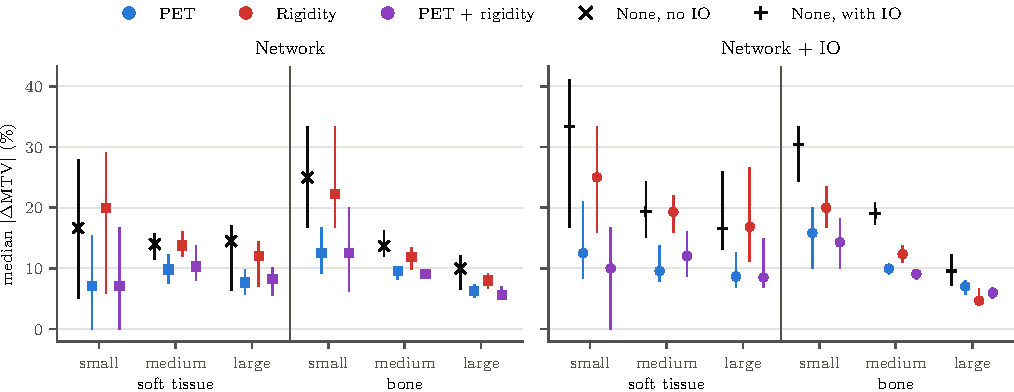
\includegraphics[width=\textwidth]{figures/lesions.pdf}
\caption{Per-lesion absolute volume change on the test set (1327 lesions from 26 patients and 30 pairs after excluding 108 components smaller than five voxels), stratified by location (soft tissue or bone-associated, with $\geq$50\,\% of the lesion on bone) and size (small $<0.5$~ml, medium $0.5$ to $<5$~ml, large $\geq5$~ml).
 Points show the median $|\Delta\mathrm{MTV}|$ per lesion; left: network output, right: instance optimization (IO) with the same losses.
 Within each size stratum, the loss groups are ordered PET, rigidity, and PET plus rigidity; squares and circles denote without and with IO, while $\times$ and $+$ denote the corresponding configurations without losses.
 Error bars: 95\,\% confidence intervals from a patient-cluster bootstrap.}
\label{fig:lesions}
\end{figure}
